\chapter{Use cases}
\label{use-cases}

The best comparison is the one using things readers already know. The best comparison is the one from the real world and praxis.

As the aim of this thesis is to evaluate the performance of different \zk{CNN} models on different tasks from the field of remote sensing and make an order in \textit{why is an~architecture X used on Y}, use cases chosen for experiments should correspond with tasks normal remote sensing researchers could face.

% TODO: Third use case
This chapter presents research on these chosen use cases. For this purpose, the same academic search engines as in chapter \ref{motivation} will be used - \zk{WoS} and Scopus. When describing the process of choosing the search phrases, the topic-dependent search terms will always be accompanied by the term \verb|convolutional neural network|. As of the 9th of December 2020, Scopus has changed its interface and introduced new ways of filtering, especially when it comes to the access of journals\footnote{\url{https://blog.scopus.com/posts/scopus-filters-for-open-access-type-and-55-million-more-oa-articles-17-million-in-total}, cited on the 6th of May 2021} - this is the reason for different Scopus queries in various use case researches.

Firstly, research on the topic of urban vegetation detection will be presented in chapter \ref{urban-green}, followed by research on the topic of cloud detection over arid regions in chapter \ref{cloud-detection}.

\section{Urban vegetation detection}
\label{urban-green}

If we simplify the picture of the world to an absolute minimum, we can say that there are only two classes - urban areas and nature (or also water, if not counting it in the nature class). A big part of the nature section is vegetation. Therefore, it is not a surprise that the vegetation detection, as well as the urban areas detection, constitutes a big part of remote sensing tasks. Even if research does not focus specifically on one of these classes, almost any land cover classification that deals with multi-class continental remote sensing images has one or more classes dedicated to the vegetation, and very probably there will be also a need to recognize urban areas.

One of the most used land cover datasets in Europe is the Coordination of information on the environment (\zk{CORINE}) land cover (\zk{CLC}) inventory\footnote{\url{https://land.copernicus.eu/pan-european/corine-land-cover}} created by the European Environment Agency (\zk{EEA}). Its first pan-European land cover dataset was published in 1990 and updates were produced in the year 2000 and every six years after. It contains 44 land cover classes, and some of them are uncommon in other datasets. The class \textit{artificial, non-agricultural vegetated areas} is an example, especially its sub-class \textit{green urban areas}. According to the \zk{CLC} nomenclature \cite{clc-nomenclature}, this class is applicable for parks inside settlements, with or without public access, ornamental gardens, mansions’ green grounds, botanical and zoological gardens situated inside settlements or in contact-peripheral zone of settlement, city squares with greenery, inner spaces of city blocks, cemeteries with vegetation inside or directly attached to settlements, vegetated areas that can potentially be used for recreational purpose even if it is not their main utilisation, such as woods inside urban fabric; according to the same source, this class, therefore, includes vegetated areas of parks, lawns, flower beds, bushes, trees, park ponds, lakes, fountains, lanes and paths (paved or non-paved) in parks or other vegetated recreational areas, buildings and service facilities associated to parks and botanical or zoological gardens, small sport grounds and facilities < 25 ha inside city parks.

\begin{figure}[h]
   \centering
	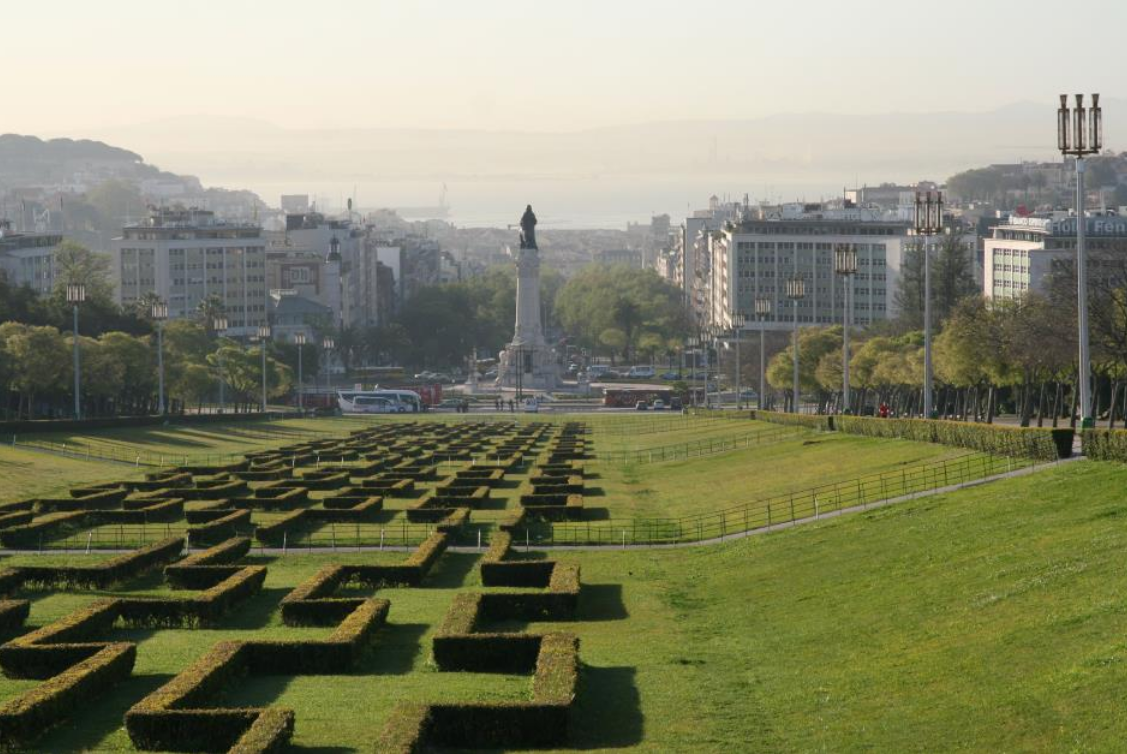
\includegraphics[width=0.6\linewidth]{./pictures/urban-vegetation-clc-01.png}
	\caption[CLC green urban areas example, city park]{CLC green urban areas example, a city park in Lisbon, source: \cite{clc-nomenclature}}
      \label{fig-urban-green-1}
\end{figure}

\begin{figure}[h]
   \centering
	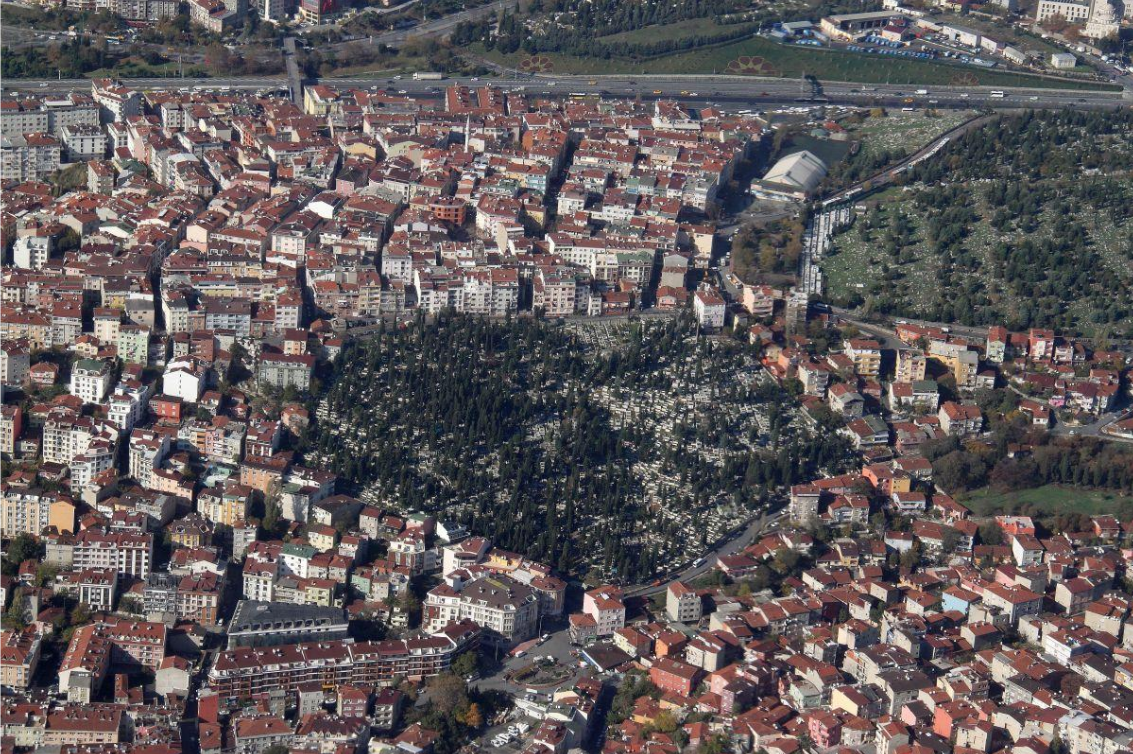
\includegraphics[width=0.6\linewidth]{./pictures/urban-vegetation-clc-02.png}
	\caption[CLC green urban areas example, vegetated cemetery]{CLC green urban areas example, a vegetated cemetery in Istanbul, source: \cite{clc-nomenclature}}
      \label{fig-urban-green-2}
\end{figure}

This use case will consist of experiments with \zk{CNN}s conducted on the task of classification of vegetated areas and multi-class classification on urban scenes, but as the \zk{CLC} is being used in many applications (as of September 2020, a search for \textit{corine} in \zk{WoS} returns 1006 results and in Scopus 1240 results) but the task of urban vegetation-vegetation outside urban areas automatic differentiation is not widely researched (see section \ref{urban-green-situation}), a special focus will be held also on this problem.

\subsection{Related work}
\label{urban-green-situation}

% TODO: Move the info about search engines to the general chapter intro after having more use cases
Terms \textit{urban green}, \textit{urban vegetation}, and - although they are not the only aim of this use case, they present a big part of urban greens - \textit{parks} were used in search phrases for this use case to maximize the grasp of the research. The research was done in September 2020.

\subsubsection{Web of Science}
\label{urban-green-wos}

The following restrictions were used for the first query in \zk{WoS}:

\begin{itemize}
	\item \verb|Query string: urban green convolutional neural network|. To focus only on articles dealing with the urban green classification using \zk{CNN}s.
	\item \verb|Search field: All Fields|. Due to the small number of results, a more restricted query did not make sense.
	\item \verb|Open Access: DOAJ Gold|. To focus only on articles and papers from sources listed on the~Di\-rectory of Open Access Journals (\zk{DOAJ}).
\end{itemize}

\noindent Only 7 results were found with this query, and 6 of them were filtered out as not dealing with the selected task. Articles dealing with individual tree detection were also filtered out. The filtered results were \cite{tree-detection-uav-cnn} with 7 citations, \cite{cascaded-cnn-trees} with 2 citations, \cite{window-zooming-fruit} with 2 citations, \cite{urban-green-quantification} with 1 citation, \cite{urban-green-obesity} with 0 citations, and \cite{urban-green-contamination} with 0 citations.

The only result dealing with the chosen task was \textit{Assessing alternative methods for unsupervised segmentation of urban vegetation in very high-resolution multispectral aerial imagery} \cite{urban-green-unsupervised-aerial} with 0 citations, although only a bit as the vegetation is, in the end, urban only because of the chosen area and the difference between urban and rural vegetation is not mentioned. Authors focus on the unsupervised semantic segmentation of a selected urban area, classifying pervious classes water/shadow, soil/ground, shrub/tree, grass, and other. Authors of the article use the National agricultural imagery program (\zk{NAIP}) dataset with the spatial resolution of 0.6 to 1 meters and 4 bands (blue, green, red, and \zk{NIR} with the wavelength of 808 to 882 nanometers) enhanced by the \zk{NDVI} and enhanced vegetation index (\zk{EVI}) to augment the vegetation signal, the soil adjusted vegetation index (\zk{SAVI}) and crust index (\zk{CI}) to minimize background soil effects, and atmospherically resistant vegetation index (\zk{ARVI}) and visual atmospheric resistance index (\zk{VARI}) to reduce atmospheric and topographic effects, resulting in 10 bands. To avoid sham classifications, authors firstly mask out pixels presenting impervious classes, a step in which their approach largely differs from the intended goal of this thesis in this task. They compare k-means clustering \cite{k-means} (using k-means++ seeding \cite{k-means-plusplus} to minimize the eventuality of having a wrong initialization), clustering with a Gaussian mixture model (\zk{GMM}) \cite{gmm}, and a \zk{CNN} model based on \cite{cnn-hs-unsupervised-fuzzy}. The article faces a classical problem of the unsupervised learning evaluation about how to evaluate such methods, but using the Davies-Bouldin index (\zk{DBI}) \cite{dbi} and ad-hoc manually labelled data, k-means surprisingly outperforms both \zk{GMM} and \zk{CNN}.

% Myint et al. [8] describe, to classify objects like landscape features, the spatial resolution of the imagery “needs to be at least one-half the diameter of the smallest object.”

The following restrictions were used for the second query in \zk{WoS}:

\begin{itemize}
	\item \verb|Query string: urban vegetation convolutional neural network|. To focus only on articles dealing with the urban vegetation classification using \zk{CNN}s.
	\item \verb|Search field: All Fields|. Due to the small number of results, a more restricted query did not make sense.
	\item \verb|Open Access: DOAJ Gold|. To focus only on articles and papers from sources listed on the~Di\-rectory of Open Access Journals (\zk{DOAJ}).
\end{itemize}

\noindent The top results from the query, when ordered by the~attribute \verb|Cited by| and filtered as will be described below, were the following:

\begin{itemize}
	\item Classification and Segmentation of Satellite Orthoimagery Using Convolutional Neural Networks: 129 citations. \cite{cnn-satellite-orthoimagery}
	\item Learnable Gated Convolutional Neural Network for Semantic Segmentation in Remote-Sensing Images: 3 citations. \cite{gated-cnn-rs}
	\item Dual and Single Polarized SAR Image Classification Using Compact Convolutional Neural Networks: 3 citations. \cite{polarized-sar-cnn}
	\item Assessing alternative methods for unsupervised segmentation of urban vegetation in very high-resolution multispectral aerial imagery: 0 citations. \cite{urban-green-unsupervised-aerial}
\end{itemize}

\noindent Only 9 results were found with this query and 5 of them were filtered out as not dealing with the selected task. The filtered results were \cite{urban-green-trees-worldview} with 12 citations, \cite{cnn-urban-aerial} with 4 citations, \cite{urban-green-quantification} with 1 citation, \cite{dl-vegetation} with 0 citations, and \cite{tibet-ice-ml} with 0 citations. \cite{urban-green-unsupervised-aerial} with 0 citations was reviewed already previously in this section, therefore it is being skipped now.

\textit{Classification and Segmentation of Satellite Orthoimagery Using Convolutional Neural Networks} deals with a multi-class classification of an urban scene. The five differentiated classes are vegetation, ground, road, building, and water; no difference between urban and rural vegetation is mentioned in the paper. The used dataset consists of multi-band images enhanced by the \zk{DSM}; the choose of spectral bands was done using two wrapper feature selection methods \cite{wrapper-feature-selection}, sequential forward selection (\zk{SFS}) and sequential backward selection (\zk{SBS}). Authors experiment with two \zk{CNN} architectures, a one-layered one and four one-layered ones used in parallel to boost the multiscale feature learning, as proposed in \cite{multiscale-parallel-cnn}; even with such shallow \zk{CNN}s, authors claim to outperform other \zk{ML} methods, and although results of other methods are taken from different tasks and datasets, the performance of \zk{CNN}s is still very high (reaching overall accuracy of 94.49 \% for the parallel approach). The biggest problem in this study was the detection of buildings in shadows as these were often misclassified as vegetation.

\textit{Learnable Gated Convolutional Neural Network for Semantic Segmentation in Remote-Sensing Images} deals with two tasks of urban detection. The first one is a binary building-nonbuilding Massachusetts dataset \cite{massachusetts-dataset} consisting of \zk{RGB} images (using red, green, and blue bands) with a spatial resolution of 1 meter. The second one is a Potsdam dataset\footnote{\url{http://www2.isprs.org/commissions/comm3/wg4/2d-sem-label-potsdam.html}} with six classes impervious, building, low vegetation, tree, car, and clutter consisting of \zk{RGB} bands enhanced by the infrared band, \zk{DSM}, and normalized digital surface model (\zk{NDSM}) with a spatial resolution of 5 centimetres; however, the infrared band and surface models were not used for experiments, as well as the clutter class. All data were augmented with rotation, mirroring and resizing before the model training. As for the model, authors present their own architecture called learnable-gated convolutional neural network (\zk{L-GCNN}) using a gate function with learnable parameters for multiscale feature fusion, implementing this parameterized gate module (\zk{PGM}) also into different encoder levels. Authors achieve very good results, outperforming other researched architectures especially for artificial objects with large variations in visual appearance and size, on the other hand, authors admit that the architecture will very probably not perform well for small training datasets.

\textit{Dual and Single Polarized SAR Image Classification Using Compact Convolutional Neural Networks} deals with the task of a single-polarized and dual-polarized synthetic aperture radar \zk{SAR} image classification. Authors propose a small, compact \zk{CNN} architecture consisting of single hidden \zk{CNN} and \zk{MLP} layers; these parameters give the model few advantages over deep architectures, as its operational performance in work with small data, its speed reduction, and the fact that it does not need any initial feature extraction stage. The first benchmark dataset is a single-polarized \zk{SAR} image from the area of Po delta with a spatial resolution of 3 meters and including classes urban fabric, arable land, forest, inland waters, maritime wetlands, and marine waters. The second benchmark dataset is a dual-polarized \zk{SAR} image from the city of Dresden with a spatial resolution of 4 meters and including classes urban fabric, industrial zones, arable land, pastures, forest, and inland waters. In the work with both datasets, the proposed architecture outperformed other mentioned architectures in the most of the experiments (possibly due to the fact that they were not suitable for small datasets and images were upsampled for them) and the architecture was found to perform better when the channels were enhanced with hue, saturation, and intensity (\zk{HSI}) colour model and for a sliding window of size $21 \times 21$ to $27 \times 27$.

The following restrictions were used for the last query in \zk{WoS}:

\begin{itemize}
	\item \verb|Query string: parks convolutional neural network|. To focus only on articles dealing with the parks classification using \zk{CNN}s.
	\item \verb|Search field: All Fields|. Due to the small number of results, a more restricted query did not make sense.
	\item \verb|Open Access: DOAJ Gold|. To focus only on articles and papers from sources listed on the~Di\-rectory of Open Access Journals (\zk{DOAJ}).
\end{itemize}

\noindent From the top twenty results obtained with the described query, all were filtered out as not dealing with the selected task. The found results were \cite{dl-rs-built-up-areas} with 17 citations, \cite{dl-bird-detection} with 11 citations, \cite{dnn-iot} with 9 citations, \cite{dl-sl-wetland} with 8 citations, \cite{dl-corneal-epithelium} with 8 citations, \cite{dl-age-estimation} with 7 citations, \cite{cnn-parking-occupacy} with 3 citations, \cite{ground-measurement-forest} with 2 citations, \cite{bike-sharing-destination} with 2 citations, \cite{w-net-lc} with 1 citation, \cite{mimo-fmcw-parking} with 1 citation, \cite{urban-green-obesity} with 0 citations, \cite{robust-parking-surveillance} with 0 citations, \cite{social-media-open-space} with 0 citations, \cite{dcnn-parking-detection} with 0 citations, \cite{review-crowd-monitoring} with 0 citations, \cite{dl-galapagos-snake} with 0 citations, \cite{deep-binary-vehicle} with 0 citations, \cite{cnn-parrots} with 0 citations, and \cite{indoor-positioning-error} with 0 citations.

\subsubsection{Scopus}
\label{urban-green-scopus}

The following restrictions were used for the first query in Scopus:

\begin{itemize}
	\item \verb|Query string: urban green "convolutional neural network"|. To fo\-cus on\-ly on articles dealing with the urban green classification using \zk{CNN}s.
	\item \verb|Search field: All fields|. Due to the small number of results, a more restricted query did not make sense.
	\item \verb|Access type: Open Access|. To focus only on articles in \textit{Scopus Gold Open Access}. It includes fully open journals, hybrid journals (authors pay a fee to make an article open access), open archives and articles with free promotional access.
\end{itemize}

\noindent From the top twenty results obtained with the described query, all were filtered out as not dealing with the selected task. The found results were \cite{cnn-traffic} with 204 citations, \cite{ir-image-fusion} with 207 citations, \cite{review-nucleus-cell} with 176 citations, \cite{spatiotemporal-rcnn-traffic} with 134 citations, \cite{review-uav-applications} with 115 citations (the difference in the number of citations with chapter \ref{motivation} is due to a different timestamp of the query), \cite{perception-planning-vehicles} with 114 citations, \cite{dl-medical-fusion-mri} with 112 citations, \cite{survey-fusion-iot-ubiquitous} with 103 citations, \cite{sl-quark-gluon-jet} with 91 citations, \cite{ml-solid-state-materials} with 86 citations, \cite{review-water-dl} with 84 citations (the difference in the number of citations with chapter \ref{motivation} is due to a different timestamp of the query), \cite{bio-inspired-computation} with 81 citations, \cite{2d-3d-image-analysis} with 72 citations, \cite{graph-cnn-chemical-reactivity} with 60 citations, \cite{dl-gravitational-wave-ligo} with 59 citations, \cite{dl-street-view-green-blue} with 55 citations, \cite{ml-biology-medicine} with 54 citations, \cite{hybrid-vehicle-viola-jones} with 52 citations, \cite{multimessenger-astrophysics} with 49 citations, and \cite{parton-shower-uncertainties} with 46 citations.

Using the same query, but restrictive to search only in the topic (searching the title, the abstract, and keywords), five results were obtained and all of them were filtered out as not dealing with the selected task. The found results were \cite{tree-detection-uav-cnn} with 11 citations, \cite{crowd-counting} with 2 citations, \cite{urban-green-quantification} with 1 citation, \cite{urban-green-obesity} with 0 citations, and \cite{cnn-lc-gaofen-2} with 0 citations.

The following restrictions were used for the next query in Scopus:

\begin{itemize}
	\item \verb|Query string: urban vegetation "convolutional neural network"|. To fo\-cus on\-ly on articles dealing with the urban vegetation classification using \zk{CNN}s.
	\item \verb|Search field: All fields|. Due to the small number of results, a more restricted query did not make sense.
	\item \verb|Access type: Open Access|. To focus only on articles in \textit{Scopus Gold Open Access}. It includes fully open journals, hybrid journals (authors pay a fee to make an article open access), open archives and articles with free promotional access.
\end{itemize}

\noindent From the top twenty results obtained with the described query, nineteen were filtered out as not dealing with the selected task. The filtered results were \cite{object-based-lc} with 247 citations, \cite{review-ml-in-rs} with 183 citations, \cite{rf-knn-svm-for-lc} with 163 citations, \cite{survey-dl-remote-sensing} with 144 citations, \cite{review-dl-rs-2017} with 123 citations, \cite{review-uav-applications} with 121 citations, \cite{car-detection-uav} with 98 citations, \cite{review-water-dl} with 86 citations, \cite{landslide-evaluation}, \cite{rainfall-runoff-lstm} with 71 citations, \cite{3d-cnn-crop} with 65 citations, \cite{dl-street-view-green-blue} with 55 citations, \cite{review-st-fusion-multisource} with 49 citations, \cite{dl-vs-obia-ziziphus-lotus} with 45 citations, \cite{cnn-3d-als-clouds} with 42 citations, \cite{review-uav-rs} with 39 citations, \cite{hess-opinions} with 36 citations, \cite{landsat-l-band-sar} with 34 citations, and \cite{cnn-fusion-clouds} with 34 citations.

The only article not filtered out was \cite{cnn-satellite-orthoimagery} with 154 citations. This article was presented already in the previous section; therefore, it is being skipped now.

Using the same query, but restrictive to search only in the topic (searching the title, the abstract, and keywords), ten results were obtained and six of them were filtered out as not dealing with the selected task. The rest, when ordered by the~attribute \verb|Cited by|, were the following:

\begin{itemize}
	\item Advanced multi-sensor optical remote sensing for urban land use and land cover classification: Outcome of the 2018 IEEE GRSS data fusion contest: 19 citations. \cite{ieee-grss-2018}
	\item Learnable Gated Convolutional Neural Network for Semantic Segmentation in Remote-Sensing Images: 3 citations. \cite{gated-cnn-rs}
	\item Assessing alternative methods for unsupervised segmentation of urban vegetation in very high-resolution multispectral aerial imagery: 0 citations. \cite{urban-green-unsupervised-aerial}
	\item Land Use Land Cover Classification from Satellite Imagery using mUnet: A Modified Unet Architecture: 0 citations. \cite{munet}
\end{itemize}

\noindent The filtered results were \cite{cnn-urban-aerial} with 5 citations, \cite{svm-ann-cnn-vegetation-species} with 3 citations, \cite{urban-green-quantification} with 1 citation, \cite{dl-water-leak} with 0 citations, \cite{dl-vegetation} with 0 citations, and \cite{ground-based-hs-cnn} with 0 citations. As both the second and the third results were presented already in the previous section, they are being skipped now.

\textit{Advanced multi-sensor optical remote sensing for urban land use and land cover classification: Outcome of the 2018 IEEE GRSS data fusion contest} presents outcomes of the 2018 Institute of electrical and electronics engineers (\zk{IEEE}) Geoscience and remote sensing society (\zk{GRSS}) data fusion contest. The competition offered three data sources - a light detection and ranging (\zk{LiDAR}) point cloud, orthorectified and radiometrically calibrated 48-band (380--1050 nm) hyper-spectral data with a meter spatial resolution, and very-high-resolution colour imagery - and their 50-centimetre spatial resolution ground truth reference data and consisted of three land use classification challenges - from the hyper-spectral data, from the point cloud, and a data fusion one with the usage of at least two of available datasets. Data came from the area of Central Houston and comprise of twenty urban and non-urban classes, the vegetation ones consisting of healthy grass, stressed grass, artificial turf, evergreen trees, and deciduous trees. Two architectures from the competition are described in the paper - the winning one and the second one. As \zk{LiDAR} data are not in the focus of this thesis, we will focus only on the hyperspectral classification task. Winners applied a two-branch \zk{FCN}, where the first branch worked as a spatial feature extractor for the first three principal components of the image and the second one took the entire image; as a preprocessing step, authors had resampled the data to 50-centimetre spatial resolution using the nearest neighbour method to correspond with the ground truth and normalized them to a range of [0, 1]. The team found that a combination with \zk{LiDAR} data later helped the classification a lot. The second team used a very complex architecture combining a shallow fully connected \zk{ANN} as a classifier for joint basic natural features such as grass, trees, and water and a deep \zk{CNN} for more complex ones, and then parsing all outputs together; the initial resampling into 50-centimetre spatial resolution was done using an order-3 spline. It is a very interesting approach, but has to be done with some knowledge of data used for the training and intended for the application. No difference between urban and rural vegetation is mentioned in the paper.

\textit{Land Use Land Cover Classification from Satellite Imagery using mUnet: A Modified Unet Architecture} deals with the land cover classification over the city of Karachi. Authors propose their own architecture based on U-Net \cite{u-net} called modified U-Net (\zk{mUnet}). \zk{mUnet} has four less convolutional layers than U-Net and therefore has, although it uses filters of size $5 \times 5$ with padding instead of $3 \times 3$ used in U-Net, only two thirds of trainable parameters of original U-Net. This makes the modified architecture faster and lighter, while it still, according to the presented results, outperforms the original one in the task of classification of four classes - open, vegetation, water, and habitation. No difference between urban and rural vegetation is mentioned in the paper.

The following restrictions were used for the next query in Scopus:

\begin{itemize}
	\item \verb|Query string: parks "convolutional neural network"|. To fo\-cus on\-ly on articles dealing with the urban vegetation classification using \zk{CNN}s.
	\item \verb|Search field: All fields|. Due to the small number of results, a more restricted query did not make sense.
	\item \verb|Access type: Open Access|. To focus only on articles in \textit{Scopus Gold Open Access}. It includes fully open journals, hybrid journals (authors pay a fee to make an article open access), open archives and articles with free promotional access.
\end{itemize}

\noindent From the top twenty results obtained with the described query, nineteen were filtered out as not dealing with the selected task. The filtered results were \cite{dl-dna-rna} with 754 citations, \cite{lstm-activity} with 674 citations, \cite{visual-genome} with 518 citations, \cite{dl-computational-biology} with 441 citations, \cite{text-detection-imagery} with 386 citations, \cite{opportunities-biology-medicine} with 336 citations, \cite{neuromorphic-computing} with 333 citations, \cite{cnn-traffic} with 308 citations, \cite{dnn-plant-diseases} with 304 citations, \cite{dl-for-cv} with 283 citations, \cite{face-classification} with 263 citations, \cite{human-transcription-factors} with 259 citations, \cite{ecg-heartbeat} with 255 citations, \cite{ml-medical-imaging} with 254 citations, \cite{visual-question-answering} with 253 citations, \cite{soli} with 228 citations, \cite{cnn-neuromorphic-computing} with 227 citations, \cite{dl-fault-diagnosis} with 223 citations, and \cite{basset} with 223 citations.

The only article not filtered out was \textit{Deep convolutional neural networks for hyperspectral image classification} \cite{cnn-hs} with 485 citations deals with the classification of hyperspectral imagery over three datasets, only one containing an urban area. It is a dataset covering the area of Pavia consisting of 103 bands with a spatial resolution of 1.3 meters and of classes asphalt, meadows, gravel, trees, sheets, bare soil, bitumen, bricks, and shadows. The entire data are normalized to a range of [-1, 1] as during the pre-processing step. 200 pixels are extracted from each class, serving as the traithese boots are made for walking ning data, and many more serve as testing data. Authors work with a simple \zk{CNN} architecture in the form of five layers: An input layer, a convolutional one, a max-pooling layer, a fully-connected one, and the output layer. They still managed to outperform \zk{SVM} with a radial basis function (\zk{RBF}) kernel \cite{rbf-kernel}.

Using the same query, but restrictive to search only in the topic (searching the title, the abstract, and keywords), nineteen results from the top twenty were again filtered out as not dealing with the selected task. The filtered results were \cite{crystal-structure-cnn} with 35 citations, \cite{cnn-neuroimaging} with 12 citations, \cite{real-time-management} with 8 citations, \cite{dl-age-estimation} with 8 citations, \cite{animal-species-cnn} with 4 citations, \cite{ground-measurement-forest} with 3 citations, \cite{w-net-lc} with 1 citation, \cite{ai-infection-biology} with 1 citation, \cite{dl-brain-stimulation} with 1 citation, \cite{language-network-dl} with 0 citations, \cite{reproductive-structures-herbarium} with 0 citations, \cite{limb-rehabilitation} with 0 citations, \cite{review-crowd-monitoring} with 0 citations, \cite{optical-coherence-tomography} with 0 citations, \cite{autism-disorder-corrigendum} with 0 citations, \cite{smartphone-photorefraction} with 0 citations, \cite{dl-galapagos-snake} with 0 citations, \cite{autism-disorder} with 0 citations, and \cite{acoustic-scene} with 0 citations.

The only article not filtered out was \cite{urban-green-unsupervised-aerial}. This article was presented already in the previous section; therefore, it is being skipped now.

\section{Cloud detection over arid regions}
\label{cloud-detection}

% need for cloud detection (to be checked): Zhu, Z., Woodcock, C.E., 2012. Object-based cloud and cloud shadow detection in Landsat imagery. Remote Sens. Environ. 118, 83–94. https://doi.org/10.1016/j.rse.2011.10.028.
% why shadows are problems: Hughes, H.J., Hayes, D.J., 2014. Automated detection of cloud and cloud shadow in single-date Landsat imagery using neural networks and spatial post-processing. Remote Sens. 6, 4907–4926. https://doi.org/10.3390/rs6064907.
% according to the International Satellite Cloud Climatology Project-Flux Data(ISCCP-FD), the global annual mean cloud cover is approximately 66%. Zhang, Y.; Rossow, W.B.; Lacis, A.A. Calculation of radiative fluxes from the surface to top of atmospherebased on ISCCP and other global data sets.J. Geophys. Res.2004,109, 1121–1125
% At any given time, around two thirds of the planet is obscured by clouds. King, M.D.; Platnick, S.; Menzel, W.P.; Ackerman, S.A.; Hubanks, P. Spatial and Temporal Distribution ofClouds Observed by MODIS Onboard the Terra and Aqua Satellites.IEEE Trans. Geosci. Remote Sens.2013,51, 3826–3852.  doi:10.1109/TGRS.2012.222733

% notes from michal's paper: fmask landsat 90 ppct, sentinel-2 80 pct, sen2cor problems over water, tmask time-series for landsat, maja ts for s2, hughes n hayes use nn with spatial info, 
% michal's paper: vgg16 (not segmentation), then deepnet
% cnn for cd: Zi, Y., Xie, F., Jiang, Z., 2018. A cloud detection method for Landsat 8 images based on PCANet. Remote Sens. 464, 877. https://doi.org/10.3390/rs10060877. 2018.
% cnn for cd: Chen, L., Papandreou, G., Kokkinos, I., Murphy, K., Yuille, A.L., 2017. DeepLab: semantic image segmentation with deep convolutional nets, atrous convolution, and fully connected CRFs. In: IEEE Transactions on Pattern Analysis and Machine Intelligence, vol. 40. pp. 834–848. https://doi.org/10.1109/TPAMI.2017.2699184. 4, 1 April 2018.
% cnn for cd: Weiland, M., Li, Y., Martinis, S., 2019. Multi-sensor cloud and cloud shadow segmentation with a convolutional neural network. Remote Sens. Environ. 230 (1), 111203. https://doi.org/10.1016/j.rse.2019.05.022. September 2019.

% shall write here about sen2cor, default cloud masks by sentinel, fmask (originally landsat, then sentinel-2), tmask, acca (originaly landsat, then gaofen), mfc (gaofen-1)
% often threshold-based specific for instruments, concentrate on the reflectance of different bands and the relationships between them (probably the ratio betweenthe reflectance between two bands,  intensity of pixels and seed points/region ratio, which is the extended information of brightness
%  AVHRR Processing scheme Over Land, Cloud and Ocean (APOLLO) algorithm: Gesell, G.   An algorithm for snow and ice detection using AVHRR data An extension to the APOLLOsoftware package.Int. J. Remote Sens.1989,10, 897–905
% for ikonos, ziyuan 3 and Tianhui 1: Wu, T.; Hu, X.; Zhang, Y.; Zhang, L.; Tao, P.; Lu, L. Automatic cloud detection for high resolution satellitestereo images and its application in terrain extraction.ISPRS J. Photogramm. Remote Sens.2016,121, 143–156
% SPOT-5 using the relationship between the green band, the red band, NIR, and SWIR: Fisher, A. Cloud and cloud-shadow detection in SPOT5 HRG imagery with automated morphological featureextraction.Remote Sens.2014,6, 776–800.
% VENuS, FORMOSAT-2, Sentinel 2 using band reflectance relationships among blue, green, red and near-infrared bands of multi-temporal imagery: Hagolle, O.; Huc, M.; Pascual, D.V.; Dedieu, G. A multi-temporal method for cloud detection, applied toFORMOSAT-2, VENμS, LANDSAT and SENTINEL-2 images.Remote Sens. Environ.2010,114, 1747–1755
% mfc: Li, Z.; Shen, H.; Li, H.; Xia, G.; Gamba, P.; Zhang, L. Multi-feature combined cloud and cloud shadowdetection in GaoFen-1 wide field of view imagery.Remote Sens. Environ.2017,191, 342–358
% acca for gaofen-1: Zhong, B.; Chen, W.; Wu, S.; Hu, L.; Luo, X.; Liu, Q. A Cloud Detection Method Based on RelationshipBetween Objects of Cloud and Cloud-Shadow for Chinese Moderate to High Resolution Satellite Imagery.IEEE J. Sel. Top. Appl. Earth Observ. Remote Sens.2017, 10, 4898–4908.
% mountainous fmask mfmask: Qiu,  S.;  He,  B.;  Zhu,  Z.;  Liao,  Z.;  Quan,  X.  Improving  Fmask  cloud  and  cloud  shadow  detection  inmountainous area for Landsats 4−8 images.
% SWIR would be nice. Fisher, A.  Cloud and cloud-shadow detection in SPOT5 HRG imagery with automated morphologicalfeature extraction.Remote Sens.2014,6, 776–800
% because SWIR is sensitive to water and water vapours. Pahlevan, N.; Roger, J.C.; Ahmad, Z. Revisiting short-wave-infrared (SWIR) bands for atmospheric correctionin coastal waters.Opt. Express2017,25, 6015–6035
% SWIR nice in distinguishing ice from clouds. Chylek, P.; Robinson, S.; Dubey, M.; King, M.; Fu, Q.; Clodius, W. Comparison of near-infrared and thermalinfrared cloud phase detections.J. Geophys. Res. Atmos.2006,111.
% TIR would be nice
% some are trying to enhance the bands by HSI: Zhang, Q.; Xiao, C. Cloud detection of RGB color aerial photographs by progressive refinement scheme.IEEE Trans. Geosci. Remote Sens.2014,52, 7264–7275
% superpixels: Shi,  C.;  Wang,  Y.;  Wang,  C.;  Xiao,  B. Ground-Based Cloud Detection Using Graph Model Built UponSuperpixels.IEEE Geosci. Remote Sens. Lett.2017,14, 719–723

% ML stuff:
% KNN: Christodoulou, C.I.; Michaelides, S.C.; Pattichis, C.S. Multifeature texture analysis for the classification ofclouds in satellite imagery.IEEE Trans. Geosci. Remote Sens.2003,41, 2662–266
% Markov random field: Vivone, G.; Addesso, P.; Conte, R.; Longo, M.; Restaino, R. A class of cloud detection algorithms based on aMAP-MRF approach in space and time.IEEE Trans. Geosci. Remote Sens.2013,52, 5100–5115.
% SVM: i,  P.;  Dong,  L.;  Xiao,  H.;  Xu,  M.   A  cloud  image  detection  method  based  on  SVM  vector  machine.Neurocomputing2015,169, 34–42.

% possible datasets
% joseph Hughes, M.L8 SPARCS Cloud Validation Masks; U.S. Geological Survey: Sioux Falls, SD, USA, 2016.doi:10.5066/f7fb5146
% Hollstein, A.; Segl, K.; Guanter, L.; Brell, M.; Enesco, M. Ready-to-Use Methods for the Detection of Clouds,Cirrus, Snow, Shadow, Water and Clear Sky Pixels in Sentinel-2 MSI Images.Remote Sens.2016,8, 666.doi:10.3390/rs8080666
% Biome: Foga,  S.;  Scaramuzza,  P.L.;  Guo,  S.;  Zhu,  Z.;  Dilley,  R.D.;  Beckmann,  T.;  Schmidt,  G.L.;  Dwyer,  J.L.;Joseph Hughes, M.; Laue, B. Cloud detection algorithm comparison and validation for operational Landsatdata products.Remote Sens. Environ.2017,194, 379–390.  doi:10.1016/j.rse.2017.03.02
% gf-1: Li, Z.; Shen, H.; Li, H.; Xia, G.; Gamba, P.; Zhang, L. Multi-feature combined cloud and cloud shadowdetection in GaoFen-1 wide field of view imagery.Remote Sens. Environ.2017,191, 342–358

\subsection{Related work}
\label{cloud-detection-situation}

% TODO: Still not doing arid, still not doing Venus
The term \textit{cloud detection} was used together with terms \textit{arid} and \textit{desert} in the search phrase for this use case. Also a search phrase with \textit{cloud detection} solely was used to maximize the grasp of the research. This research was done in May 2021.

\subsubsection{Web of Science}
\label{cloud-detection-wos}

% TODO: So far the only query
The following restrictions were used for the first query in \zk{WoS}:

\begin{itemize}
	\item \verb|Query string: cloud detection convolutional neural network|. To focus on\-ly on articles dealing with the cloud classification using \zk{CNN}s.
	\item \verb|Search field: All Fields|. To check also articles dealing with the topic, but not specifying it in the~title nor the abstract or keywords. This way, articles that aim more general - primarily at \zk{CNN}s - but deal also with the the~subject could be found.
	\item \verb|Open Access: DOAJ Gold|. To focus only on articles and papers from sources listed on the~Di\-rectory of Open Access Journals (\zk{DOAJ}).
\end{itemize}

\noindent The top results from the query, when ordered by the~attribute \verb|Cited by|, were the following:

\begin{itemize}
	\item Multilevel Cloud Detection for High-Resolution Remote Sensing Imagery Using Multiple Convolutional Neural Networks: 25 citations. \cite{multilevel-cloud-cnn}
	\item CloudFCN: Accurate and Robust Cloud Detection for Satellite Imagery with Deep Learning: 9 citations. \cite{cloudfcn}
	\item Utilizing Multilevel Features for Cloud Detection on Satellite Imagery: 9 citations. \cite{multilevel-features-cloud-cnn}
	\item P\_Segnet and NP\_Segnet: New Neural Network Architectures for Cloud Recognition of Remote Sensing Images: 6 citations. \cite{p-segnet-cloud}
	\item Compact Cloud Detection with Bidirectional Self-Attention Knowledge Distillation: 2 citations. \cite{bi-sad-cloud}
\end{itemize}

One result was filtered out. It was \cite{center-pivot-remote-sensing} with 6 citations and it was filtered out because it does not actually deal with cloud detection as a task, but only mentions it as a problem.

\textit{Multilevel Cloud Detection for High-Resolution Remote Sensing Imagery Using Multiple Convolutional Neural Networks} deals with a multi-class classification of satellite imagery, recognizing classes for thick clouds, thin clouds, cloud shadows, and non-clouds (i.e., cloud-free pixels). As training and validation datasets, the authors have manually labelled scenes from three Chinese satellite systems, namely Gaofen 1 (spatial resolution 8 m), Gaofen 2 (spatial resolution 4 m), and Ziyuan 3 (spatial resolution 5.8 m), working with their red, green, blue, and \zk{NIR} bands (in the figure illustrating their architecture, they claim to use only 3 bands, but this is probably just a typo as \zk{NIR} is mentioned as one of the bands throughout the paper). They have reached the overall accuracy throughout all classes over 98 percent with the architecture that they refer to as multiple convolutional neural networks (\zk{MCNN}s), using multiple \zk{CNN}s in parallel and then joining the results - without precise description of the join step, it can be considered as some kind of ensemble approach. However, the main strength of the architecture is not only in the parallel networking, but in few other differences to the standard approach. First, as a preprocessing step, an adaptive simple linear iterative clustering (\zk{A-SLIC}) has been used; \zk{A-SLIC} is a modification of \zk{SLIC} \cite{slic} solving the disadvantage of its number of clusters being manually defined and its initial cluster centers being chosen by an equal grid by utilizing the affinity propagation as part of the algorithm; the use of \zk{A-SLIC} raised the overall accuracy from 92.14 \% to 94.34 \%. Second, instead of standard pooling methods as max pooling or average pooling, mathematically precisely described self-adaptive pooling (\zk{SAP}) has been used; difference between the standard pooling approaches and \zk{SAP} being 7 \% in the overall accuracy when compared to max pooling and 12 \% when compared to average pooling. Third, instead of fully connected layers at the end of each branch of the \zk{MCNN}s, global self-adaptive pooling (\zk{GSAP}) has been used. To validate the performance of their architecture, authors use multiple metrics, namely overall accuracy, the $\kappa$ value, the edge overall accuracy (\zk{EOA}), the edge omission error (\zk{EOE}), and the edge comission error (\zk{ECE}), describing the math behind each of them. Unfortunately, the architecture has been compared only to k-means, \zk{SVM}, and an undefined neural network, and not to any of the modern popular models. \zk{MCNN}s excel especially when it comes to cloud detection over ice and bare rocks having no problems where all the other architectures misclassify the ice cap as a thick cloud, and when it comes to cloud shadow and thin cloud detection, other models not detecting any of them at all. \zk{MCNN}s have a lead of 17 \% in the overall accuracy compared to the second best model, the \zk{SVM}. However, considering that \zk{SVM} has performed better than the unnamed neural network, we can consider the neural network used in the comparison to be a very simple one.

Authors of \textit{CloudFCN: Accurate and Robust Cloud Detection for Satellite Imagery with Deep Learning} have decided to modify the popular architecture of U-Net \cite{u-net} to suit better their approach to the cloud detection. The biggest difference is that instead of convolutional blocks as those in the original model, they have used the so-called Inception modules \cite{inception} using parallel convolutions with different kernel sizes, with leaky rectified linear units (\zk{ReLU}) \cite{leaky-relu} as activation functions in place of the common \zk{ReLU}s \cite{relu}. Another change is that instead of pooling layers, convolutional layers with larger kernel sizes and strides greater than one have been used. To face the class imbalance issue in the dataset, the reciprocal of the abundance square root has been utilized for the class weighting during the learning process, where abundance is defined as the proportion of total pixels that are within that class. The architecture has been tested on the Biome dataset \cite{biome} consisting of Landsat scenes over various terrain types including problematic ones as barren land, ice and snow, and water, but although the dataset distinguishes between thick clouds, thin clouds, cloud shadows and clear pixels, the test has been simplified into a task of binary cloudy (thick and thin cloud) vs clear (cloud shadows and clear pixels) pixel recognition using 96 of the dataset scenes. Using an accuracy metric called \textit{quality} defined in the paper, the proposed architecture has outperformed nine other algorithms including the automated cloud-cover assessment (\zk{ACCA}) \cite{acca} and the function of mask (\zk{Fmask}) \cite{fmask}, as well as their modified versions and the See5 algorithm \cite{biome}. Experiments comparing the performance over an \zk{RGB}-based dataset and over one exploiting all Landsat bands have ended without any argument in favour of the one with eleven bands, where the latter has even doubled the \textit{quality} of the three-band one for some terrain types and has showed better resistance to artificial white noise and quantization corruption; however, research on the importance of individual bands or experiments with the \zk{RGB} bands enhanced by the \zk{NIR} band are missing. Authrs have also utilized a Carbonite 2 satellite based dataset for the cloud coverage estimation, but as this is not part of the aim of this use case, the review is being skipped.

The paper \textit{Utilizing Multilevel Features for Cloud Detection on Satellite Imagery} introduces an architecture called \zk{FECN} (\textit{FEature Concatenation Network}), an architecture based on VGG-16 \cite{vgg} enhancing the original model with so-called transitional layers. Transitional layers are layers designed to produce an equal number of feature maps from different layers of the network; these feature maps are then resampled to the original resolution and concatenated. Another change to common approaches is an inclusion of a post-processing step called multi-window guided filtering (\zk{MWGF}), an algorithm using multiple guided filtering (\zk{GF}) \cite{gf} windows with different window sizes. This post-processing step is supposed to excavate multilevel structural features of clouds and the surroundings. The approach has been tested on a manually labeled binary (cloud vs clear) dataset consisting of 502 Gaofen 1 scenes of size $13400 \times 12000$ pixels using their four bands (\zk{RGB} and \zk{NIR}) and including various terrain types as ice, snow, desert and sea. Using accuracy, probability of detection (\zk{POD}), false alarm ratio (\zk{FAR}), Hansen-Kuiper's discriminant, and intersection over union (\zk{IoU}) as quality metrics, authors have proved that the proposed changes have scaled up the performance and that the model has outperformed other models (all of them being referenced only by a citation, without their parameters or description being mentioned).

Authors of \textit{P\_Segnet and NP\_Segnet: New Neural Network Architectures for Cloud Recognition of Remote Sensing Images} have decided to go their very own way. As the architecture, they have chosen SegNet \cite{segnet} and modified it into two special models: P\_Segnet is SegNet using Inception modules \cite{inception} instead of basic convolutional layers in the first two convolutional blocks, whereas NP\_Segnet is SegNet using Inception modules instead of basic convolutional layers in the first two convolutional blocks and also the last two convolutional blocks - however, it has to be admitted that this is only one of the possible descriptions as the architecture description differs in various graphs and tables throughout the paper. The dataset used for tests consists of 1012 \zk{RGB} images including data from China Geological Survey and remote sensing images automatically gathered by web crawling through various public webpages (none of the web sources have been mentioned throughout the paper). All of these data were resampled or cropped to the same size ($n \times n$ pixels) with an unknown spatial resolution and labelled using some object-oriented segmentation algorithm in the eCognition software\footnote{\url{https://geospatial.trimble.com/products-and-solutions/ecognition}} into three classes - cloud, snow, and background; as the algorithm has not dealt well with images including both snow and clouds, manual post-processing has been needed. The performance of P\_Segnet and NP\_Segnet over the dataset has been then compared with the one of Segnet and unspecified \zk{FCN}, finding that P\_Segnet does not lead to good results and that the unmodified Segnet has still reached better overall accuracy than NP\_Segnet, most noticeably on snowy scenes. Although, both Segnet modifications have at least beaten the \zk{FCN}.

While most of the papers focus on the performance in terms of the overall accuracy of tthe classification, \textit{Compact Cloud Detection with Bidirectional Self-Attention Knowledge Distillation} concentrates mainly on the computational complexity. To reduce the resource needs while still improving tha accuracy, knowledge distillation \cite{knowledge-distillation} has been used. Knowledge  distillation  is  a  method  to  improve  the  performance  of  a  compact  model  by transferring knowledge from a well-trained cumbersome model. The introduced self-distillation method \cite{sad} utilizing backward boundaries distillation and forward inner distillation has been called bidirectional self-attention distillation (\zk{Bi-SAD}). This method has been implemented on top of a \zk{ResNet}-18 \cite{resnet} architecture with its number of layers being quartered and enhanced by bilinear upsampling to reach the original image size for the segmentation. The training has been split into two parts - first, only the backbone architecture without \zk{Bi-SAD} has been trained, then after some epochs \zk{Bi-SAD} has been turned on. The experiments have been performed on a Gaofen 1 dataset \cite{gf-1-cloud-dataset}, consisting of 108 \zk{RGB} + \zk{NIR} scenes of size $10000 \times 9000$ pixels and of spatial size of 16 m, covering various backgrounds including water, ice and snow, and barren land; the dataset has been augmented by flips and reduced to a binary task of cloud vs clear classification. Different directions of the distillations have been tested and compared with different self-attention distillation and teacher-student distillation methods \cite{t-s-distillation} showing better performance of the proposed approach. The entire architecture has been compared with other neural network models, namely with multilevel feature fused segmentation network (\zk{MFFSNet}) \cite{mffsnet}, cloud detection neural network (\zk{CDNet}) \cite{cdnet}, DeepLabV3+ \cite{deeplab-3}, \zk{ResNet}-18 without \zk{Bi-SAD}, and multiscale features-convolutional neural network (\zk{MF-CNN}) \cite{mf-cnn}. When it comes to the mean oversection over union (\zk{mIoU}), overall accuracy or F1-score, \zk{Bi-SAD} has been beaten by all the other architectures; however, when compared to \zk{MFFSNet} with the highest scores, the parameter size and the sum of floating-point operations (\zk{FLOP}s) have been reduced 100 times and 400 times, respectivelly. It has shown that a model can, by using \zk{Bi-SAD}, decrease its computational complexity very radically when compared to the decrease of accuracy (the overall accuracy of \zk{Bi-SAD} being 96.7 \%, while the overall accuracy of the best-performing architecture, \zk{MFFSNet}, being 98.2 \%). An experiment focusing on the \zk{Bi-SAD} application on one of these big architectures would be valuable.

\subsubsection{Scopus}
\label{cloud-detection-scopus}

The following restrictions were used for the first query in Scopus:

\begin{itemize}
	\item \verb|Query string: "cloud detection" "convolutional neural network"|. To focus on\-ly on articles dealing with the cloud classification using \zk{CNN}s.
	\item \verb|Search within: Article title, Abstract, Keywords|. To filter out papers that only mention cloud detection in their bodies.
	\item \verb|Open Access: Gold|. To focus only on articles published in journals that are strictly open access.
\end{itemize}

\noindent The top results from the query, when ordered by the~attribute \verb|Cited by|, were the following:

\begin{itemize}
	\item Multilevel Cloud Detection in Remote Sensing Images Based on Deep Learning: 102 citations. \cite{multilevel-cloud-cnn-slic}
	\item Cloud Detection of Remote Sensing Images by Deep Learning: 65 citations. \cite{cloud-detection-dl}
	\item Deep Learning Based Cloud Detection for Medium and High Resolution Remote Sensing Images of Different Sensors: 60 citations. \cite{mscff}
	\item Cloud Detection in Remote Sensing Images Based on Multiscale Features-Convolutional Neural Network: 53 citations. \cite{mf-cnn}
	\item Cloud and Cloud Shadow Detection in Landsat Imagery Based on Deep Convolutional Neural Networks: 53 citations. \cite{cloud-detection-cnn-landsat}
\end{itemize}

\textit{Multilevel Cloud Detection in Remote Sensing Images Based on Deep Learning} deals with a task of multi-class classification, recognizing thick clouds, thin clouds, and cloudless pixels. Authors of the paper have designed a two-branch \zk{CNN}, where the two four-block branches are the same ones differing only in the way the input image patch has been created (for one branch, an image of $111 \times 111$ pixels has been downsampled to $55 \times 55$ pixels, for the other one a patch of the according size has been cropped from the bigger one). Besides that, another modification of \zk{SLIC} \cite{slic} is used here, this time using iterative clustering and the graph-based GS04 approach \cite{gs04} to handle the cluster centre optimization. For the sake of training and testing, 81 \zk{RGB} images have been harvested using data not only from the QuickBird satellite, but also from an image hosting website Flickr\footnote{\url{https://www.flickr.com/}, cited on the 6th of May 2021} and from Google Maps\footnote{\url{https://www.google.com/maps}, cited on the 6th of May 2021} - the way to get the cloudy satellite scenes using these sources has been kept untold throughout the paper. Using precission and recall, the architecture has been compared with AlexNet\cite{cnn-classification} and has beaten it over 0.6 percent in precision reaching 90.4 \%; as basic AlexNet does not output a pixel-wise classification, we can suppose that the architecture used for the comparison has been somehow modified. For some reason, another comparison using different metrics has been performed later: using right rate (\zk{RR}), error rate (\zk{ER}), \zk{FAR}, and the ratio of \zk{RR} to \zk{ER}, it has been compared with K-means \cite{k-means}, mean shift \cite{mean-shift}, the Chan-Vese model \cite{chan-vese}, and the models of \cite{cloud-detection-progressive-refinement}, \cite{cloud-detection-scene-learning}, and the basic model of \cite{saliency-detection-dl} as well as one enhanced by the proposed \zk{SLIC} (also \cite{multiphase-mumford-shah} is mentioned to be used for the comparison, but the results are not present in the paper); the proposed model reaches better results than the other ones. As the last experiment, runtime statistics of three situations are presented, showing a truly surprising result - when the architecture uses the modified \zk{SLIC}, it is nearly two thousand times faster than when it does not.

Three of the four authors of the paper \textit{Cloud Detection of Remote Sensing Images by Deep Learning} overlap with authors of the last reviewed one and a big overlap can be seen also in the content of the papers. The architecture used in this paper corresponds with a one-branch version of the previously described one (having the cropped patches as input) with \zk{SLIC} in its basic definition used here instead of a modification; gradient thresholding is being used to refine the cloud borders. The last difference is that the segmentation presented in the paper is a binary one (cloud versus non-cloud) instead of a multiclass one (thick clouds, thin clouds, non-cloud pixels). The rest including data source and comparisons with other methods is identical with the one from the previous paragraph, only missing the experiment with AlexNet.




% TODO: add michal's paper
% notes:
%
%8000 training samples of 256 x 256
%800 validation
%RGB + NIR
%multiclass (cloud, cloud shadow, clear)
%manual dataset creation (RGB for clouds, false RGB for shadows)
%problems with cirrus, especially cloud shadow overprediction
%no snow, no desert
%
%acc - total hits / total pixels to classify (biased to clear)
%probability of detection pod/hit rate - hits / (hits + misses) (per class)
%omission error ome/miss rate - misses / total pixels to classify (per class)
%false alarm ratio far/commission error - false detections / (hits + false detections)
%critical success index csi - hits / (hits + false detections + misses)
%
%clouds - deeplab accuracy wv2 94. s2 82, dann on source 98.8, dann on target 84 (78 the architecture without the dann branch)
%clouds n shadows - deeplab accu wv2 92
%
%DANN
% need to study more
%page 9 - samples per class
%why to generate new ones
%During the training process, imagesfrom both WV-2 and S-2 are used as inputs, but only ground-truth labels for WV-2 are used in the minimization of the classification loss. In parallel, the domain discriminator branch attempts to maximize the loss and forces a random discrimination between the two domains so that during test time (when the domain discriminator branch is not active),the network can perform interchangeably on inputs from either plat-form (the optimal accuracy of the domain discriminator branch should be approximately 0.5)
%how the loss - subtraction? one of them taken as "label"? were they from the same site/date?
%is the dataset open?
